\chapter{Discrete Distributions}

\section{Random Variables}

\subsection{Introduction to Random Variables}

\begin{definition}[Random Variable]\index{Random Variable}
    A \term{random variable} is a real-valued function that assigns a numerical value to each event in the sample space $\Omega$ arising from a random experiment. A random variable $X$ is a \bred{real-valued function} $X : \Omega \to \mathbb{R}$ such that for every $\omega \in \Omega$, $X(\omega) = x \in \mathbb{R}$. It is a mapping from the sample space to the real numbers.
\end{definition}

\begin{example}
    Consider the random experiment of tossing a coin. 

    \begin{itemize}
        \item $\Omega = \{ H, T \}$
        \item Let $X$ be the RV denoting the outcome of a toss. We ca define $X$ such that $X(H) = 1$, $X(T) = 0$ essentially converting each outcome into a number. 
        \item By convention, we will denote random variables with capital letters, and a particular (unknown value) of a random variable with its lower case equivalent. i.e. for a random variable $X$, a particular value of this RV would be denoted by $x$.
    \end{itemize}
\end{example}

\begin{definition}[Discrete Random Variable]\index{Discrete Random Variable}\index{Continuous Random Variable}
    A \term{discrete} of a random variable $X$ is one tha can take on only a finite number of a countably infinite number of possible values $x$. A random variable $X$ is \term{continuous} if its domain is an interval of real numbers. 
\end{definition}

\begin{definition}[Probability Mass Function]\index{Probability Mass Function}
    A \term{probability mass function} (PMF) of a discrete random variable is one that assigns a probability to each value $x \in C$ such that 
    \begin{itemize}
        \item $0 \le P(X = x) \le 1$
        \item $\sum_{x \in X} P(X = x) = 1$
    \end{itemize}
\end{definition}

\begin{example} 
    Below are some examples of random variables. 

    \textbf{Discrete RV Examples}
    
    \begin{itemize}
        \item The number of defects in a day's production of car parts 
        \item The number of new arrivals in a queue 
        \item The status of your internet service: online or offline 
        \item The number of students online at a particular time
    \end{itemize}

    \textbf{Continuous RV Examples}

    \begin{itemize}
        \item The weight of a randomly selected individual 
        \item The time it takes to load a video 
        \item The temperature in the morning of a random day
    \end{itemize}
\end{example}

\begin{example}
    Determine the value of $k$ such that $f(x) = \frac{kx^2 - x + 2}{4}$ will be a valid probability mass function for $X = \{ 0, 1, 2, 3, 4 \}$.

    \begin{center}
        \begin{tabular}{c | c c c c c}
            $X$        & 0             & 1               & 2              & 3                & 4                 \\
            \hline
            $P(X = x)$ & $\frac{2}{4}$ & $\frac{k+1}{4}$ & $\frac{4k}{4}$ & $\frac{9k-1}{4}$ & $\frac{16k-2}{4}$
        \end{tabular}
    \end{center}

    We need $\sum_{x=0}^4 P(X = x) = 1$. That is, 
    $\begin{aligned}[t]
        \frac{2 + (k+1) + (4k) + (9k-1) + (16k-2)}{4} & = 1            \\
        30k                                           & = 4            \\
        k                                             & = \frac{2}{15}
    \end{aligned}$

    Thus, $k$ must be $\frac{2}{15}$ for $\sum_{x \in X} P(X = x) = 1$. 

    \begin{center}
        \begin{tabular}{c | c c c c c}
            $X$        & 0             & 1               & 2              & 3              & 4              \\
            \hline
            $P(X = x)$ & $\frac{1}{2}$ & $\frac{17}{60}$ & $\frac{2}{15}$ & $\frac{1}{20}$ & $\frac{1}{30}$
        \end{tabular}
    \end{center}
\end{example}

\begin{example}
    A factory producing computer parts sends out a shipment of $10$ parts of which $3$ are defective. Find the probability mass function for the number of defectives a customer will get if the first customer randomly purchases $4$ computer parts.

    Let $D$ be the number of defectives purchased. 

    $D = \{ 0, 1, 2, 3 \}$. 

    \begin{itemize}
        \item $P(D = 0) = \frac{_7C_4}{_{10}C_4}$
        \item $P(D = 1) = \frac{_3C_1 \times _7C_3}{_{10}C_4}$
        \item $P(D = 1) = \frac{_3C_2 \times _7C_2}{_{10}C_4}$
        \item $P(D = 1) = \frac{_3C_3 \times _7C_1}{_{10}C_4}$
    \end{itemize}

    We may conclude that $P(D = d) = \frac{_3C_d \times _7C_{4-d}}{_{10}C_4}$. 
\end{example}

\begin{example}
    A quiz consists of $10$ true/false problems. A student takes the quiz by randomly selecting the answers. Examine the graph of the probability mass function and describe the behaviour of the random number of correct answers X.

    For discrete distribution, we use bar charts. The bins are $0, 1, 2, 3, \dots, 10$, which are discrete. Histograms, on the other hand, has bins that span a continuous interval, for example, $[0, 1), [1, 2), [2, 3), \dots$. 

    \begin{itemize}
        \item $4, 5, 6$ have the highest probability mass, meaning they are the most \itblue{likely}; 
        \item $0, 1, 2, 8, 9, 10$ have the lowest probability mass, meaning that they are the most \itblue{unlikely};
        \item $3$ and $7$ lie between \itblue{likely} and \itblue{unlikely}.
    \end{itemize}

    \begin{center} 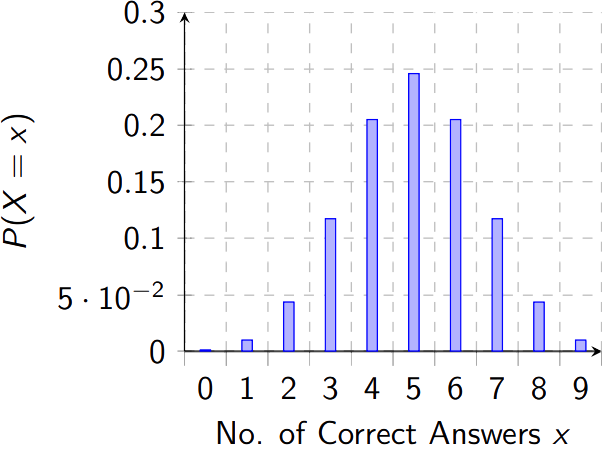
\includegraphics[width=0.5\linewidth]{PmfExamplesTFQuiz.png} \end{center}
\end{example}

\subsection{Characteristics of Random Variables}

Both the PMF and CDF describe the exact distribution of a random quantity. Distributions have two useful characteristics that are often used in statistics:

\begin{itemize}
    \item \term{Expected Value}: The long run/theoretical average. If a random experiment were to be conducted $n$ times, then as $n \to \infty$ then the average of outcomes converges to the expected value. This is often denoted as $\mu$.
    \item \term{Variance} or \term{Standard Deviation}: Are measures of the spread and variability of a random variable. Standard deviation is the square root of variance. Variance is often denoted as $\sigma^2$ and SD as $\sigma$.
\end{itemize}

\begin{definition}[Expected Value]\index{Expected Value}
    The \term{expected value} of a discrete random quantity $X$ is defined to be $$\mu = E(X) = \sum_{x \in X} x \cdot P(X = x)$$

    For a given transformation of $X$, $g(X)$, $E(g(x))$ can be found by $$E(g(x)) = \sum_{x \in X} g(x) \cdot P(X = x)$$

    Note that $E(g(x)) \neq g(E(X))$ except when $g(X)$ is a linear transformation. 
\end{definition}

\textbf{Review of Summation Rules}

\begin{itemize}
    \item $\sum_{i=1}^n c = n \cdot c$ for a constant $c$
    \item $\sum_{i=1}^n c \cdot x_i = c \cdot \left( \sum_{i=1}^n x_i \right)$
    \item $\sum_{i=1}^n i = \frac{n \cdot (n+1)}{2}$
\end{itemize}

\begin{example}
    A mining company needs a type of drill bit for a project. It is known through historical data that these drill bits for similar projects will last $2$, $4$, or $7$ hours with probabilities $0.1$, $0.7$, and $0.2$. How long do they expect each drill bit to last, on average?

    Let $L$ be the longevity of a random drill bit.

    \begin{center}
        \begin{tabular}{c | c c c}
            $l$        & 2     & 4     & 7     \\
            \hline
            $P(L = l)$ & $0.1$ & $0.7$ & $0.2$
        \end{tabular}
    \end{center}

    $\begin{aligned}[t]
        E(L) & = \sum_{l \in L} l \cdot P(L = l)         \\
             & = 2 \cdot 0.1 + 4 \cdot 0.7 + 7 \cdot 0.2 \\
             & = 4.4 \text{ hours}
    \end{aligned}$

    $\therefore$ on average, the drill bits will last $4.4$ hours.
\end{example}

\textbf{Properties of Expectation}

For any constants $a$, $b$, and discrete variables $X$, the following are true.

\begin{itemize}
    \item $E(a) = 0$

    \item $E(X + a) = E(X) + a = \mu + a$. 

    Increase in $x \in X$ will shift the centre / average by the same amount. 

    \item $E(aX) = a \cdot E(X) = a \cdot \mu$
    
    \begin{proof}
        Take $g(X) = aX$. Then, $\begin{aligned}[t]
            E(g(x)) & = \sum_{x \in X} g(x) \cdot P(X = x) \\
                    & = \sum_{x \in X} ax \cdot P(X \in x) \\
                    & = a \sum_{x \in X} x \cdot P(X = x)  \\
                    & = a \cdot \color{red} E(x)           \\
                    & = a \cdot \mu
        \end{aligned}$
        
        That is, $E(aX) = a \cdot E(X) = a \cdot \mu$. 
    \end{proof}

    \item $E(aX + b) = a \cdot E(X) + b = a \cdot \mu + b$

    \begin{proof}
        Take $g(X) = aX + b$. $g(x)$ is a linear transformation of $X$. 

        $E(g(x)) = g(E(x))$ if $g(X)$ is a linear transformation of $X$. 
        
        Thus, $E(aX + b) = a \cdot E(X) + b = a \cdot \mu + b$. 
    \end{proof}

    \item $E(X + Y) = E(X) + E(Y)$. 

    \item $E(XY) \neq E(x) \cdot E(Y)$ \bred{unless} $X$ and $Y$ are \itblue{independent}. 
\end{itemize}

\begin{definition}[Variance]\index{Variance}\index{Standard Deriviation}
    For a discrete variable $X$, the \term{variance} of $X$ is defined to be $$\sigma^2 = V(X) = E((X - \mu)^2) = \sum_{x \in X} (x - \mu)^2 \cdot P(X = x)$$ 
    Variance captures the spread in $units^2$. The standard deviation, $\sigma = \sqrt{\text{variance}}$ is a measure of spread in the same units as the random variable $X$. 
\end{definition}

\begin{example}
    A mining company needs a type of drill bit for a project. It is known through historical data that these drill bits for similar projects will last $2$, $4$, or $7$ hours with probabilities $0.1$, $0.7$, and $0.2$. Find the variance and standard deviation in the longevity of this type of drill bit. Interpret the values

    Let $L$ be the longevity of a random drill bit.

    We also found $\mu = 4.4$

    \begin{center}
        \begin{tabular}{c | c c c}
            $l$           & 2                & 4                & 7                \\
            \hline
            $P(L = l)$    & $0.1$            & $0.7$            & $0.2$            \\
            $(l - \mu)^2$ & $(2-4.4)^2=5.76$ & $(4-4.4)^2=0.16$ & $(7-4.4)^2=6.76$
        \end{tabular}
    \end{center}

    $\begin{aligned}[t]
        V(L) & = {\sigma_L}^2                                         \\
             & = \sum_{l \in L} (l - \mu)^2 \cdot P(L = l)        \\
             & = 5.76 \cdot 0.1 + 0.16 \cdot 0.7 + 6.76 \cdot 0.2 \\
             & = 2.04 \text{ hours}^2
    \end{aligned}$

    Then, $\begin{aligned}[t]
        SD(L) = \sqrt{V(L)} & = \sigma_L                  \\
                            & = \sqrt{2.04}               \\
                            & \approx 1.4283 \text{ hours}
    \end{aligned}$

    On average, the longevity of the drill bits will vary by about 1.43 hours from the average. Typically, we expect the longevity to be between $(4.4 - 1.4283, 4.4+1.4283) = (2.97, 5.83)$ hours. 
\end{example}

\textbf{Properties of Variance}

For any constants $a$, $b$, and discrete variables $X$, the following are true.

\begin{itemize}
    \item $V(a) = a$

    Constants do not vary. 

    \item $V(X + a) = V(X) = \sigma^2$

    If the spread of $X$ is $V(X)$, increasing each $x \in X$ will not change how spread out the random variable is. 

    \item $V(aX) = a^2 \cdot V(X) = a^2 \cdot \sigma^2$
    
    \begin{proof}
        $\begin{aligned}[t]
            V(aX) & = E \left( (aX - E(aX))^2 \right)        \\
                  & = E \left( (ax - a\mu)^2 \right)         \\
                  & = E \left( (a \cdot (x - \mu))^2 \right) \\
                  & = E \left( a^2 \cdot (x - \mu)^2 \right) \\
                  & = a^2 \cdot E \left( (x - \mu)^2 \right) \\
                  & = a^2 \cdot V(X)
                  & = a^2 \cdot \sigma^2
        \end{aligned}$
        
        That is, $V(aX) = a^2 \cdot V(X) = a^2 \cdot \sigma^2$. 
    \end{proof}

    \item $V(aX + b) = a^2 \cdot V(X) = a^2 \cdot \sigma^2$

    \item $V(X + Y) \neq V(x) + V(Y)$ \bred{unless} $X$ and $Y$ are \itblue{independent}. 
\end{itemize}

\begin{example}
    A mining company needs a type of drill bit for a project. It is known through historical data that these drill bits for similar projects will last $2$, $4$, or $7$ hours with probabilities $0.1$, $0.7$, and $0.2$. 

    \begin{enumerate}[label=\alph*)]
        \item If they ordered $10$ drill bits of the same type for replacement once one drill bit fails, how long can they expect these drill bits to last for this project?

        Let $L$ be the longevity of drill bits. 

        $\begin{aligned}[t]
            E(L_1 + L_2 + \cdots + L_{10}) & = \sum_{i=1}^{10} E(L_i)       \\
                                           & = 4.4 + 4.4 + \cdots + 4.4     \\
                                           & = 44 \text{ hours}
        \end{aligned}$

        {~~~}
        
        \item Find the variance and standard deviation in the longevity for the $10$ drill bits that were ordered.

        All drill bits are independent, so $\begin{aligned}[t]
            V(L_1 + L_2 + \cdots + L_{10} & = \sum_{i=1}^{10} V(L_i)      \\
                                          & = 2.04 + 2.04 + \cdots + 2.04 \\
                                          & = 20.4 \text{ hours}^2
        \end{aligned}$

        Then, $\begin{aligned}[t]
            SD(L_1 + L_2 + \cdots + L_{10}) & = \sqrt{20.4}              \\
                                            & \approx 4.52 \text{ hours}
        \end{aligned}$

        On average, they can expect the drill bits to last $44 \pm 4.52$ hours. That is, from $39.48$ hours to $48.52$ hours. 
    \end{enumerate}
\end{example}

An alternative method for calculating the variance of a discrete random variable $X$ with PMF $f(x)$ can be derived as follows:
\begin{align*}
    E((X - \mu)^2) & = E(X^2 - 2X\mu + \mu^2)             \\
                   & = E(X^2) - 2\mu \cdot E(X) + \mu^2   \\
                   & = E(X^2) - 2E(X) \cdot E(X) + E(X)^2 \\
                   & = E(X^2) - E(X)^2
\end{align*}

This breakdown is ``allowed'' since $\mu = E(X)$ is an unknown \bred{constant}. 

Note that $E(X^2) \neq E(X)^2$. To compute $E(X^2)$, refer back to the definition of expected value. That is, $$E(X^2) = \sum_{x \in X} x^2 \cdot f(x)$$

\section{Cumulative Distribution Function}

The probability behaviour of a random variable can be represented in many ways, such as with the probability mass function. Another representation is with the \term{cumulative distribution function}.

\begin{definition}[Cumulative Distribution Function]\index{Cumulative Distribution Function}
    The \term{cumulative distribution function} (CDF) $F(x)$ of a discrete random variable with probability mass function $P(x)$ or $f(x)$ is a function that returns the cumulative (total) probability up to and including $X = x$. $$F(b) = P(X \le b) = \sum_{x \in \{ x \le b \}} P(x)$$ The domain of the CDF is always over the set of real numbers! As such, CDFs are often represented as a piecewise function.
\end{definition}

\begin{example}
    Find the cumulative distribution function for PMF below:

    \begin{center}
        \begin{tabular}{ c | c c c c}
            $x$        & $0$           & $1$           & $2$            & $3$            \\
            \hline
            $P(X = x)$ & $\frac{1}{6}$ & $\frac{1}{2}$ & $\frac{3}{10}$ & $\frac{1}{30}$ \\
        \end{tabular}
    \end{center}
    
    $$F(x) = \begin{cases}
        0                        & \text{if } x < 0       \\
        \textstyle \frac{1}{6}   & \text{if } 0 \le x < 1 \\
        \textstyle \frac{2}{3}   & \text{if } 1 \le x < 2 \\
        \textstyle \frac{29}{30} & \text{if } 2 \le x < 3 \\
        1                        & \text{if } x \ge 3
    \end{cases}$$
\end{example}

\subsection{Properties of CDF}

\textbf{CDF of a Discrete Random Variable}

For a discrete random variable $X$ with CDF $F(X)$:

\begin{enumerate} \everymath{\displaystyle}
    \item The graph of the CDF will be a \bred{non-decreasing step-function}. That is for $a < b$, $F(a) \le F(b)$. 
    \item The graph of the CDF is \bred{right continuous}. That is, $\lim_{x \to c^+} F(x) = F(c)$. 
    \item $\lim_{x \to \infty} F(x) = 1$
    \item $\lim_{x \to -\infty} F(x) = -1$
\end{enumerate}

\begin{example}
    A discrete random variable $X$ has cumulative distribution function defined by
    $$F(X) = \begin{cases}
        0    & x < 0       \\
        0.3  & 0 \le x < 3 \\
        0.55 & 3 \le x < 5 \\
        0.88 & 5 \le x < 4 \\
        1    & x \ge 7
    \end{cases}$$

    \begin{enumerate}[label=\alph*)]
        \item Plot the CDF. 
        
        \begin{center} 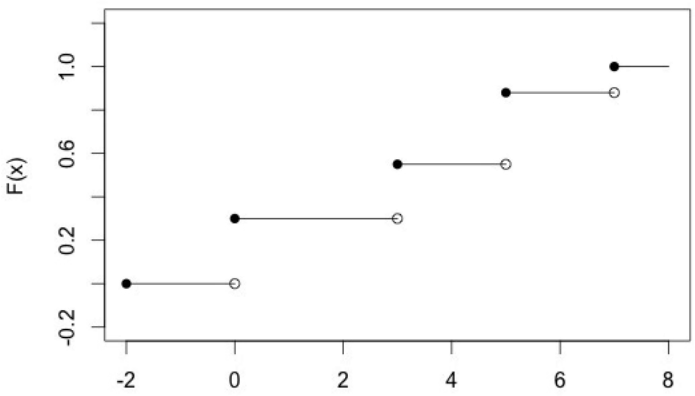
\includegraphics[width=0.75\linewidth]{CdfExamplesReadingProbabilities.png} \end{center}

        \item What is the probability that $X$ is less than $5$?

        $P(x < 5) = 0.55$

        \item What is the probability of $X = 2$?

        $\begin{aligned}[t]
            P(X = 2) & = P(X \le 2) - P(X < 2) \\
                     & = 0.3 - 0.3             \\
                     & = 0
        \end{aligned}$

        Note that $P(X = 2) = 0$ has no changes to CDF on interval of $[0, 3)$. The only outcomes with probability mass are $X = 0$ and $X = 3$. 
    \end{enumerate}
\end{example}

\subsection{Chebyshev's Inequality}

For a given random variable $X$, $\mu_X$ and ${\sigma^2}_X$ are measures of two features of the distribution of $X$: it's `centre' and it's spread. How can we use these two values to better understand the distribution of $X$, especially in the absence of the exact distribution such as the probability mass function (PMF) or the cumulative distribution function (CDF)?

\begin{theorem}[Markov's Inequality]\index{Markov's Inequality}
    Let $X$ be a \bred{non-negative} random variable with mean $E(X)$/ Then, for some constant $\color{red} a > 0$, $$P(X \ge a) \le \frac{E(X)}{a}$$
\end{theorem}

\begin{proof}
    Since $X$ is a non-negative random variable, $\forall x \in X$, $x \ge 0$. 

    Then, $\begin{aligned}[t]
        E(X) & = \sum_{x \in X} x \cdot P(X = x)                                 \\
             & = \sum_{x < a} x \cdot P(X = x) + \sum_{x \ge a} x \cdot P(X = x) \\
             & \ge \sum_{x \ge a} x \cdot P(X = x)                               \\
             & \ge \sum_{x \ge a} a \cdot P(X = x) & \text{since } x \ge a       \\
             & = a \cdot \sum_{x \ge a} P(X = x)                                 \\
             & = a \cdot P(x \ge a)
    \end{aligned}$

    That is, $\begin{aligned}[t]
        E(X)           & \ge a \cdot P(X \ge a) \\
        \frac{E(X)}{a} & \ge P(X \ge a)
    \end{aligned}$
\end{proof}

\begin{theorem}[Chebyshev's Inequality]\index{Chebyshev's Inequality}
    Let $X$ be a random variable with mean (expected value) $\mu$ and finite variance $\sigma^2$. Then for any positive $k$, $$P(|x - \mu| {\color{red}~<~} k\sigma) \ge 1 - \frac{1}{k^2}$$

    Chebyshev's Inequality applies to all discrete distributions with \bred{finite} $E(X)$ and $V(X)$ for the random variable $X$. 
\end{theorem}

\begin{proof}
    $\begin{aligned}[t]
        P(|X - \mu| < k\sigma) & = P((x - \mu)^2 < k^2\sigma^2)         & \text{since RV's are non-nagative and } k > 0 \\
                               & = 1 - (P((x - \mu)^2 \ge k^2\sigma^2))
    \end{aligned}$

    By Markov's Inequality, for a non-negative random variable $X$ and a positive constant $a$, $P(X \ge a) \le \frac{E(x)}{a}$, $a > 0$. Consider $(X - \mu)^2 > 0$ as $x$ and $k^2\sigma^2 > 0$ as $a$ in Markov's Inequality, we have $\begin{aligned}[t]
        P((x - \mu)^2 \ge k^2\sigma^2) \ge \frac{E((x - \mu)^2)}{k^2\sigma^2} & = \frac{\sigma^2}{k^2\sigma^2} \\
                                                                              & = \frac{1}{k^2}
    \end{aligned}$

    That is, $P(|X - \mu| < k\sigma) \ge 1 - \frac{1}{k^2}$. 
\end{proof}

\begin{example}
    Based on past data, the average daily number of tech support requests at a local call centre is 115 with a standard deviation of 10 calls.

    \begin{enumerate}[label=\alph*)]
        \item What can be said about the fraction of days on which the number of calls received is between 100 and 130?
        
        \begin{itemize}
            \item Distribution info: missing 
            \item We are given: $\mu = 115$, $r = 10$
        \end{itemize}

        Let $C$ be the random number of daily calls. 

        $\begin{aligned}[t]
            P(100 \le C \le 130) & = P(-15 \le C - 115 \le 15) \\
                                 & = P(-15 \le C - \mu \le 15) \\
                                 & = P(|C - \mu| \le 15) \\
                                 & = P(|C - \mu| < 16) \\
                                 & = P(|C - \mu| < 1.6\sigma) \\
                                 & \ge 1 - \frac{1}{1.6} = 0.6094
        \end{aligned}$

        $\therefore$ At least $60.94\%$ of the time they will have between 100 to 130 calls a day. 

        \item What number of calls can they expect to receive at least $90\%$ of the time?

        We want to find the number of $\sigma$ that correspond to an interval that has at least $90\%$ chance of occurring. 
        
        $P(|X - \mu| < k\sigma) = 1 - \frac{1}{k^2} = 90\%$

        That is, $\begin{aligned}[t]
            1 - \frac{1}{k^2} & = 0.90        \\
            0.1               & = \frac{1}{k} \\
            k^2               & = 10          \\
            k                 & = \sqrt{10}
        \end{aligned}$

        For all distributions, more than $90\%$ of the outcomes lie within $\sqrt{10} \approx 3.16$ standard derivation of its mean. 

        $(115 - k\sigma, 115 + k\sigma) = (115 - \sqrt{10} \cdot 10, 115 + \sqrt{10} \cdot 10) \approx (83.38, 146.62)$

        $\therefore$ They can expect to receive $[83, 147]$ number of calls at least $90\%$ of the time. 
    \end{enumerate}
\end{example}

\section{Common Discrete Distributions}

\subsection{Binomial Distribution}

\begin{definition}[Bernoulli Trials]\index{Bernoulli Trials}
    A \term{Bernoulli trial} is a random experiment consisting of exactly one trial involving two possible outcomes, often called a \itblue{success} or a \itblue{failure}. Let $X$ be the outcome of a Bernoulli trial where 
    $$\begin{aligned}[t]
        X = 0 & \text{ if the outcome is a failure} \\
        X = 1 & \text{ if the outcome is a success}
    \end{aligned}$$

    We define $p$ to be the probability of \bred{success}, and $q = 1 - p$ to be the probability of \bred{failure}. The \itblue{probability mass function} is then $$f(x) = p^x \cdot (1 - p)^{1 - x}$$
\end{definition}

\begin{example}[Bernoulli Trials]
    Below are some examples of Bernoulli trials. 

    \begin{itemize}
        \item Whether a randomly selected part is defective 
        \item Whether there is an error in a line of code 
        \item Whether a randomly selected individual is taller than 5'7'' 
        \item Whether a switch is in the on or off proposition
        \item Whether your lotto ticket is the winning number
    \end{itemize}
\end{example}

\begin{example}
    Consider a multiple choice quiz $4$ questions. A student selects an answer at random for each question, and each question is a Bernoulli experiment: the student either guesses correctly ($1$) or incorrectly ($0$). The sum of these four Bernoulli experiments will then be the random number of correct answers for a student that completes a similar quiz in this way. Our sample space is: 
    $$\Omega = \left\{ \cmark \cmark \cmark \cmark, \cmark \cmark \cmark \xmark, \cmark \cmark \xmark \cmark, \cmark \xmark \cmark \cmark, \xmark \cmark \cmark \cmark, \cmark \cmark \xmark \xmark, \cmark \xmark \cmark \xmark, \xmark \cmark \cmark \xmark, \xmark \cmark \xmark \cmark, \xmark \xmark \cmark \cmark, \cmark \xmark \xmark \cmark, \right.$$
    $$\left. \xmark \xmark \xmark \cmark, \xmark \xmark \cmark \xmark, \xmark \cmark \xmark \xmark, \cmark \xmark \xmark \xmark, \xmark \xmark \xmark \xmark \right\}$$

    Suppose these MCQs have four options each, and each question only has one correct option. Find the following probabilities. 

    \begin{enumerate}[label=\alph*)]
        \item Guessing each question correctly. 

        $P(\cmark \cmark \cmark \cmark) = \frac{1}{4} \cdot \frac{1}{4} \cdot \frac{1}{4} \cdot \frac{1}{4} = \frac{1}{4^4}$

        \item Guessing each question incorrectly. 

        $P(\xmark \xmark \xmark \xmark) = \frac{3}{4} \cdot \frac{3}{4} \cdot \frac{3}{4} \cdot \frac{3}{4} = \frac{3^4}{4^4}$
        \item Guessing exactly $2$ questions correctly. 

        $P(\cmark \cmark \xmark \xmark) = \frac{1}{4} \cdot \frac{1}{4} \cdot \frac{3}{4} \cdot \frac{3}{4} = \frac{3^2}{4^4}$

        $P(2 \text{ correct}) = _4C_2 \cdot \frac{3^2}{4^4}$
    \end{enumerate}
\end{example}

Often, we are interested in modeling the number of successes among multiple trials instead of the results of a single trial:

\begin{definition}[Binomial Distribution]\index{Binomial Distribution}
    A \term{Binomial experiment} consists of $n$ independent and identical Bernoulli trials. The probability of success, $p$, is fixed for each trial. 

    {~~~}

    Let $X$ be the random variable representing the number of successes among the $n$ trials. Then $X$ can be modeled by the binomial distribution with parameters $n$ and $p$, denoted as $X \sim \mathrm{Bin}(n, p)$. The binomial distribution has probability mass function: $$P(X = x) = \binom{n}{x} \cdot p^x \cdot (1 - p)^{n - x}$$ If $X \sim \mathrm{Bin}(n, p)$, we can show that $E(X) = np$ and $V(X) = np(1 - p)$
\end{definition}

\begin{example}[Binomial Experiments]
    Below are some examples of Binomial experiments. 

    \begin{itemize}
        \item The number of people who tried the dalgona candy challenge following `Squid Game'
        \item The number number of randomly selected students who started playing Animal Crossing in 2020
        \item The number of games won out of $7$ independent games with the same opponent
    \end{itemize}
\end{example}

\begin{example}
    While studying by a window, you find yourself noticing many cars at a nearby intersection that fail to fully come to a stop at the stop sign before passing through the intersection. Based on your months of data, you reliably calculate the probability of drivers failing to do a complete stop to be $70\%$. Assuming the stopping behaviour of each car is independent of all others, find the probability that among $20$ randomly observed cars that...

    \begin{enumerate}[label=\alph*)]
        \item Exactly $5$ will come to a complete stop? 
        
        Let $S$ be the number of cars that stop. 

        $S \sim Bin(n = 20, p = 0.3)$. 

        {~~~}
        
        $\begin{aligned}[t]
            P(S = 5) & = \binom{20}{5} \cdot 0.3^5 \cdot (1 - 0.3)^{20-5}              \\
                     & = \frac{20!}{(20-5)! \cdot 5!} \cdot 0.3^5 \cdot 0.7^{15} \\
                     & \approx 0.1789
        \end{aligned}$

        \item At least $3$ will come to a complete stop?
        
        $\begin{aligned}[t]
            P(S \ge 3)
             & = \sum_{s = 3}^{20} \binom{20}{s} \cdot 0.3^s \cdot (1 - 0.3)^{20-s}                                                                    & \text{(direct)}   \\
             & = 1 - P(S < 3)                                                                                                                          & \text{(indirect)} \\
             & = 1 - P(S \le 2)                                                                                                                                            \\
             & = 1 - \left( \binom{20}{0} \cdot 0.7^{20} + \binom{20}{1} \cdot 0.3^1 \cdot 0.7^{19} + \binom{20}{2} \cdot 0.3^2 \cdot 0.7^{18} \right)                     \\
             & \approx 0.9645
        \end{aligned}$

        \item At most $3$ will come to a complete stop?
        
        $\begin{aligned}[t]
            P(S \le 3) & = P(S = 0) + P(S = 1) + P(S = 2) + P(S = 3)                                                                                                                     \\
                       & = \binom{20}{0} \cdot 0.7^{20} + \binom{20}{1} \cdot 0.3^1 \cdot 0.7^{19} + \binom{20}{2} \cdot 0.3^2 \cdot 0.7^{18} + \binom{20}{3} \cdot 0.3^3 \cdot 0.7^{17} \\
                       & \approx 0.1071
        \end{aligned}$
    \end{enumerate}
\end{example}

\begin{example}
    A  local hospital has several backup generators to support critical technologies in the event of a power outage or failure. Each backup generator is identical in make, and operate independently of others. Suppose each backup generator has a $20\%$ chance of failing when used. How many generators should be installed so that the system has at least a $99.5\%$ probability of functioning in the event of a power outage?

    Let $n$ be the number of generators (a fixed quantity).

    Let $G$ be the number of generators that functions. 

    $G \sim Bin(n, p = 0.8)$. 

    We want to find $n$ such that $P(G \ge 1) \ge 99.5\%$. 

    That is, by the indirect method, we need $\begin{aligned}[t]
        P(G = 0) & \le 0.005 \\
        \binom{n}{0} \cdot 0.2^n \le 0.005 \\
        0.2^n \le 0.005 \\
        n \ge 3.29
    \end{aligned}$

    $\therefore$ At least $4$ generators should be installed. 
\end{example}

\subsection{Poisson Distribution}

Consider modeling of the number of Shiba, $D$, spotted at a nearby park over any 1 day with a probability model. (How is this different from a Binomial model if it still models the number of `successes'?)

\begin{center} 
\includegraphics[width=0.25\linewidth]{doge.jpg} \end{center}

This is \bred{not} a binomial distribution, as trials are \itblue{discrete}, while time is \itblue{continuous}! 

Let's try to formulate this problem so it resembles a Binomial model: first we will arbitrarily divide the 1 day into $n$ equally-sized time interval with the following properties for any one interval:

\begin{itemize}
    \item $P(D = 1) = p$
    \item $P(D = 0) = 1 - p$
    \item $P(D > 1) = 0$ (i.e. the event of Shiba sighting is ``rare'')
\end{itemize}

Let us also assume that each time interval behaves independently, and the average (mean) number of Shiba sightings per day is fixed and denoted by $\lambda$. 

Based on the construction and assumptions, we have $n$ independent trials with equal probabilities of ``success'' $p$. This can be modeled as a binomial distribution where $D \sim Bin(n, p)$, which has an expected values of $E(D) = np$. 

Since the mean number of daily sightings is constant, 

\begin{itemize}
    \item $E(D) = np = \lambda$, and $p = \frac{\lambda}{n}$
    \item The number of time intervals is arbitrarily decided, neither $n$ nor $p$ are known.
    \item In order to ensure daily average $\lambda = np$ remains constant, as $n$ increases, $p$ must decrease so that $np$ remains unchanged
\end{itemize}

We'll get more accurate probabilities of daily sightings in a day if we allow each time interval to shrink to $0$ (not too different from using Riemann sums to approximate area under continuous curves!). Let's see how the binomial PMF behaves as $n \to \infty$ and $p \to 0$.

The resulting function will model the \itblue{probability of $D$ number of Shiba sightings} over a \itblue{continuous period of 1 day}.

Let $D$ be the number of Shiba sighted in ``n'' sub-intervals.

$D \sim Bin(n, p = \frac{\lambda}{n})$. 

$E(D) = np = \lambda$. 

$\begin{aligned}[t]
    P(D = d)
     & = \lim_{n \to \infty} \binom{n}{d} \cdot p^d \cdot (1 - p)^{n - d} \\
     & = \lim_{n \to \infty} \frac{n!}{(n - d)! \cdot d!} \cdot \left( \frac{\lambda}{n} \right)^d \cdot \left( 1 - \frac{\lambda}{n} \right)^{n - d} \\
     & = \frac{\lambda^d}{d!} \lim_{n \to \infty} \frac{n(n-1)(n-2)\cdots(n-d+1)\cancel{(n-d)!}}{\cancel{(n-d)!}} \cdot \frac{1}{n^d} \left( 1 - \frac{\lambda}{n} \right)^{n-d} \\
     & = \frac{\lambda^d}{d!} \lim_{n \to \infty} \frac{n}{n} \times \frac{n-1}{n} \times \frac{n-2}{n} \times \cdots \times \frac{n-d+1}{n} \cdot \left( 1 - \frac{\lambda}{n} \right)^{n-d} \\
     & = \frac{\lambda^d}{d!} \lim_{n \to \infty} \left( 1 \right) \left( 1 - \frac{1}{n} \right) \left( 1 - \frac{2}{n} \right) \cdots \left(1 - \frac{d-1}{n} \right) \left( 1 - \frac{\lambda}{n} \right)^{n-d} \\
     & = \frac{\lambda^d}{d!} \lim_{n \to \infty} \left( 1 - \frac{\lambda}{n} \right)^{n-d} \\
     & = \frac{\lambda^d}{d!} \lim_{n \to \infty} \left( 1 - \frac{\lambda}{n} \right)^n \cancelto{1}{\left( 1 - \frac{\lambda}{n} \right)^{-d}} \\
     & = \frac{\lambda^d}{d!}  \cdot e^{-\lambda} \qquad \text{as } \lim_{n \to \infty} \left( 1 - \frac{\lambda}{n} \right)^n = e^{-\lambda} \\
     & = \frac{\lambda^d e^{-\lambda}}{d!}
\end{aligned}$

\begin{definition}[Poisson Distribution]\index{Poisson Distribution}
    A discrete random variable $X$ denoting the number of (sometimes rare) events of interest in an interval, with the mean number of occurrences per unit interval denoted by $\lambda$, is \term{Poisson Distributed} if it has the probability mass function $$P(X = x) = \frac{\lambda^x e^{-\lambda}}{x!}$$

    $X$ has expectation $E(X) = \lambda$ and variance $V(X) = \lambda$. 
\end{definition}

Note that $\lambda$ is also called the \term{rare parameter} as it describes the average \itblue{rate of occurrance} of the event. $\lambda$ should always be adjusted for the time interval being considered. 

Poisson distribution is appropriate for discrete random variables that count the number of occurrences in a \bred{continuous interval} where

\begin{itemize}
    \item No more than one occurrence can occur simultaneously 
    \item Non-overlapping intervals have occurrences that behave independently 
    \item Expected number of occurrences in each fixed time interval is constant
\end{itemize}

As suggested in the construction of the Poisson distribution, this distribution can be used to approximate binomial probabilities where $n$ is large and $p$ is small. The approximation improves as $n$ increases and/or $p$ decreases. The advantage here is that Poisson distribution can be easier to compute since it doesn't involve the $\binom{n}{x}$ factor in its PMF. 

What does a Poisson distribution look like? Generally unimodal and right-skewed, there is greater likelihood in observing values near but less than the mean $\lambda = 4$.

\begin{center} 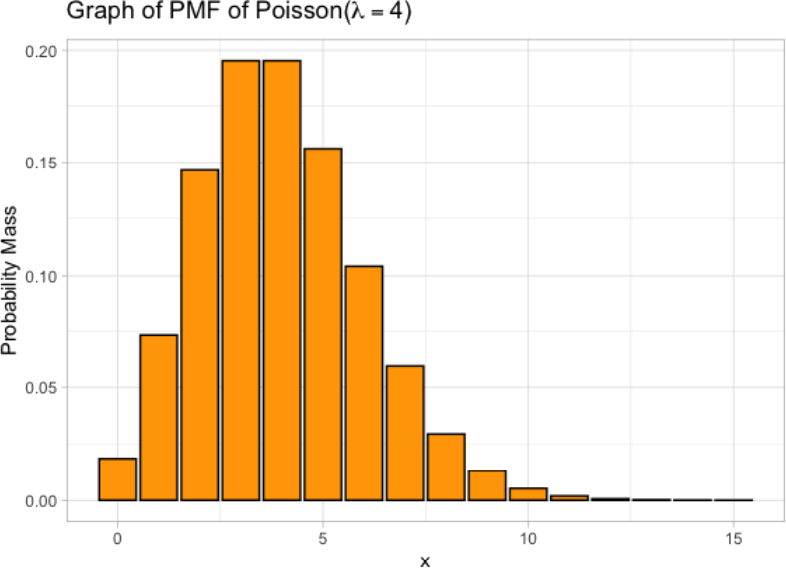
\includegraphics[width=0.75\linewidth]{PoissonDistributionPlot.png} \end{center}

\begin{example}
    An area of a forest as on average $6$ trees per $100$ m\textsuperscript{2}. 

    \begin{enumerate}[label=\alph*)]
        \item Do the assumptions for a Poisson model seem appropriate for modeling tree distribution in a forest
        
        \begin{itemize}
            \item Two simulations trees (two trees occupying the same spot) is $0$
            \item Could reasonably assume that the number of trees per area is independent
        \end{itemize}

        \item What is the probability of having at least $1$ tree in a $100$ m\textsuperscript{2} area? 
        
        Let $T$ be the number of trees per $100$ m\textsuperscript{2}. 

        $T \sim Pois(\lambda = 6)$. 

        Using the indirect method, $\begin{aligned}[t]
            P(T \ge 1) & = 1 - P(T = 0)              \\
                       & = 1 - \frac{6^0 e^{-6}}{0!} \\
                       & \approx 0.9975
        \end{aligned}$

        $\therefore$ There is $99.75\%$ change of having at least $1$ tree in a $100$ m\textsuperscript{2} area. 
    \end{enumerate}
\end{example}

\begin{example}
    The number of car repairs $R$ that arrive at a mechanic can be well modeled by a Poisson random variable with a mean of $3t$, where $t$ denotes the time in hours of operating hours. The average profit per repair is given by $Y = 85R^2 - 60t$. Assuming that vehicle arrival occurs independently,

    \begin{enumerate}[label=\alph*)]
        \item What is the probability that in a $10$ hour workday, they will service between $28$ to $31$ cars? 

        We can reasonably model $R \sim Pois(\lambda = 3 \cdot 10 = 30)$. 

        Then, $\begin{aligned}[t]
            P(28 \le R \le 31)
             & = \sum_{r=28}^{31} P(R = r)                                                                                             \\
             & = \frac{30^{28} e^{-30}}{28!} + \frac{30^{29} e^{-30}}{29!} + \frac{30^{30} e^{-30}}{30!} + \frac{30^{31} e^{-30}}{31!} \\
             & \approx 0.2858
        \end{aligned}$

        $\therefore$ $28.58\%$ of the time they will service between $28$ to $31$ cars. 

        \item What is the corresponding profit earned for the cars serviced in a)? 

        $Y = 85R^2 - 60 \cdot 10 = 86R^2 - 600$ with $R \in [28, 31]$.

        That is, $y \in [85 \cdot 28^2 - 600, 85 \cdot 31^2 - 600] = [66040, 81085]$

        $\therefore$ They are expected to earn from $\$66,040$ to $\$81,085$. 

        \item What is the expected profit for a typical $8$ hour workday?

        $R \sim Pois(\lambda = 3 \cdot 8 = 24)$
        
        $\begin{aligned}[t]
            E(Y) & = E(85R^2 - 60 \cdot 8) \\
                 & = E(85R^2 - 480) \\
                 & = 85 E(R^2) - 480 \\
        \end{aligned}$

        Since $V(R) = E(R^2) - E(R)^2$, $E(R^2) = V(R) + E(R)^2 = \lambda + \lambda^2 = 24 + 24^2$. 

        Then, $\begin{aligned}[t]
            E(Y) & = 85 (24 + 24^2) - 480 \\
                 & = \$50,520
        \end{aligned}$

        $\therefore$ The expected profit for a typcail $8$ hour workday is $\$50,520$. 

        \item Suppose that you know that in an 8 hour workday, $E(R^4) = 416,472$. Determine the variance in profit. Can you determine what interval of profits they can expect to earn with at least $75\%$ probability?

        $R \sim Pois(24)$. 

        $E(Y) = 50,520$

        $\begin{aligned}[t]
            V(Y) & = V(85R^2 - 480) = 85^2 \cdot V(R^2)  \\
                 & = 85^2 \cdot (E((R^2)^2) - E(R^2)^2)  \\
                 & = 85^2 \cdot (416,472 - (24 + 24^2)^2) \\
                 & = \$^2 408,010,200
        \end{aligned}$

        {~~~}

        $\sigma_Y = \sqrt{V(Y)} \approx \$20,199.26$

        By Chebyshev, $P(|Y - \mu_Y| < k\sigma_Y) \ge 1 - \frac{1}{k^2}$, and we want $1 - \frac{1}{k^2} = \frac{3}{4}$. That is, $k = 2$. 

        $y \in (50520 - 2(20199.26), 50520 + 2(20199.26)) = (10121.48, 90918.52)$

        $\therefore$ They are expected to earn within $(10121.48, 90918.52)$ with at least $75\%$ probability. 
    \end{enumerate}
\end{example}

\subsection{Geometric Distribution}

The geometric distribution models the probability of observing some number of \bred{consecutive failed trials before a ``success''} is observed. The trials are
independent and identical Bernoulli trials with fixed probability of success, $p$.

\begin{definition}[Geometric Distribution]\index{Memoryless Property}
    Let $X$ be the random variable representing the \itblue{number of failures before the \bred{first} success}. The probability, $p$, is fixed for each trial.
    $$P(X = x) = (1 - p)^x \cdot p$$

    A geometric distribution has expectation $E(X) = \frac{1 - p}{p}$ and variance $V(X) = \frac{1 - p}{p^2}$. 
\end{definition}

Note that $P(X \ge k) = q^k$, that is, if the number of trials is more than $k$, then the first $k$ trials must have all been failures. 

\begin{example}
    What is the probability you ask $3$ people \bred{before} you find someone born in December. You may assume that every month is equally likely to be a birth month.

    $\left( \frac{11}{12} \right)^3 \cdot \left( \frac{1}{12} \right)$

    How many people do you expect to have to ask before finding someone born in December? What is the expected total number of people surveyed?

    Total people $=$ number of failures $+ 1$

    $\begin{aligned}[t]
        E(X + 1) & = E(X) + 1 \\
                 & = \frac{1 - \frac{1}{12}}{\frac{1}{12}} + 1 \\
                 & = 12
    \end{aligned}$
\end{example}

\begin{definition}[Memoryless Property]\index{Memoryless Property}
    The geometric distribution has one additional property. It is a \term{memoryless distribution}. Suppose you have observed $j$ consecutive failures. The probability that we will observe at least another $k$ failures given that the first $j$ must be failures is the probability of observing k failures. In other words: $$P(X > j + k ~|~ x \ge j) = P(X > k)$$
\end{definition}

\begin{example}[Memoryless Property]
    The probability that a component will function for more than 5 years if it is already 2 years old is the same as the probability that it functions for more than 3 years (this is obviously unrealistic, but an example of memoryless property).
\end{example}

\begin{example}
    What is the probability that it takes at least $8$ rolls of a fair die before you roll a 6, if you did not roll a 6 in the first $4$ rolls?

    Let $D$ be the number of dice rolls before rolling a 6 \footnote{If $D = 1$, then we roll a $6$ on the second trial}. 

    $\begin{aligned}[t]
        P(D \ge 8 | D \ge 4) & = P(D \ge 8 - 4) \\
                             & = \left( \frac{5}{6} \right)^4 \\
                             & \approx 48.23 \%
    \end{aligned}$
\end{example}

\subsection{Negative Binomial Distribution}

Negative binomial random variables model the number of failed attempts before we observe a total of r successes.

The random variable can model either the number of failures or the total number of trials. Note that the two are linear shifts of each other: $$n(\text{failure}) + (\text{`r' successes}) = n(\text{trials})$$ Since the last success is guaranteed in the last trial, we can reduce the problem to finding the probability of $(r - 1)$ successes in the first $(x + r - 1)$ trials. This type of random variable $X$ has a \{term{negative binomial distribution}.

\begin{definition}[Negative Binomial Distribution]
    Let $X$ be the number of failures before $r$\textsuperscript{th} success. Each trial is an independent and identical (i.i.d) Bernoulli trial with p probability of success. 
    $$P(X = x) = \binom{x + r - 1}{r - 1} \cdot p^r \cdot (1 - p)^x$$

    A negative binomial distribution has expectation $E(X) = \frac{r(1-p)}{p}$ and variance $V(X) = \frac{r(1-p)}{p^2}$. 

    Note that if we model $Y$ to be the number of trials to achieve rth success, then we have a success in the $Y$\textsuperscript{th} trial, $Y - r$ failures and $r - 1$ successes among the first $Y - 1$ trials is $$P(Y = y) = \binom{y - 1}{r - 1} \cdot p^r \cdot (1 - p)^{y-r}$$
\end{definition}

\begin{example}[Negative Binomial Distribution]
    Below are examples of Negative Binomial Distributions.

    \begin{itemize}
        \item The number of losing lotto numbers selected before you have 6 winning numbers 
        \item The total numbers you have selected to achieve 6 winning numbers 
        \item The number of tails before getting 4 heads in consecutive coin tosses 
        \item The number of times you toss a coin to get 4 heads 
    \end{itemize}
\end{example}

\begin{example}
    Find the probability that you will have to survey $Y = D_1 + D_2 + D_3 = 10$ people NOT born in December before you have a total of $3$ people born in December (i.e. that you survey a total of $10 + 3$ people to find a total of $3$ December babies).
    $$\cmark \cmark \xmark \xmark \xmark \xmark \xmark \xmark \xmark \xmark \xmark \xmark | \cmark$$

    In order for 10 non-December individuals to be surveyed before this is fulfilled, this tells you that then 13th person is born in December, while 2 of the first 12 people are born in December.

    $\begin{aligned}[t]
        P(\text{Survey } 10 \text{ failures before } 3 \text{ successes}) 
         & = \binom{10 + 3 - 1}{3 - 1} \cdot \left( \frac{1}{2} \right)^3 \cdot \left( 1 - \frac{1}{12} \right)^{10} \\
         & = \binom{12}{2} \cdot \left( \frac{1}{2} \right)^3 \cdot \left( \frac{11}{12} \right)^{10}                \\
         & \approx 1.6 \%
    \end{aligned}$
\end{example}

\subsection{Hypergeometric Distribution}

A hypergeometric distribution can be used to calculate the probability of selecting $k$ ``successes'' out of $n$ selections \bred{when the pool of selection $N$ is small}. In other words, 

\begin{itemize}
    \item You have a population of size $N$ made up of subpopulations: ``successes'' and ``failures''. 
    \item You are randomly selecting a group of $n$ from this population (without replacement) and observing the number of ``successes'' in your group of $n$. 
    \item Example: Tagging wildlife to be tracked over several years to observe population growth, territory expansion, etc.
\end{itemize}

If the pool of selection $N$ is large relative to $n$, then the probability can be approximated using a binomial distribution.

\begin{itemize}
    \item Sampling without replacement, the probability of subsequent selections is not greatly impacted
    \item We can model this with ``n'' trials, and $p = \frac{k}{N}$
\end{itemize}

\begin{example}
    Consider the following example, where $N$ is big versus $N$ is small. 

    \begin{itemize}
        \item We have a lot of $5000$ items, $10\%$ of which are known to be defective. Find the probability of observing at least three defective items in a random selection of $10$ items.

        Let $D$ be the number of deffectives. 

        $D \sim Hypergeometric(5000, n = 10, k = 500)$

        $\begin{aligned}[t]
            P(D \ge 3) 
             & = 1 - P(D \le 2) \\
             & = 1 - \frac{\binom{4500}{10}}{\binom{5000}{10}} - \frac{\binom{500}{1} \cdot \binom{4500}{9}}{\binom{5000}{10}} - \frac{\binom{500}{2} \cdot \binom{4500}{8}}{\binom{5000}{10}} \\
             & = 7.00 \%
        \end{aligned}$

        \item We have a lot of $50$ items, $10\%$ of which are known to be defective. Find the probability of observing at least three defective items in a random selection of 10 items.

        Let $D$ be the number of deffectives. 

        $D \sim Hypergeometric(50, n = 10, k = 5)$

        $\begin{aligned}[t]
            P(D \ge 3) 
             & = 1 - P(D \le 2) \\
             & = 1 - \frac{\binom{45}{10}}{\binom{50}{10}} - \frac{\binom{5}{1} \cdot \binom{45}{9}}{\binom{50}{10}} - \frac{\binom{5}{2} \cdot \binom{45}{8}}{\binom{50}{10}} \\
             & \approx 4.83 \%
        \end{aligned}$

        \item Approximate probability ysing binomial distribution for both, since $D \sim Bin(n = 10, p = 0.10)$, $P(D \ge 3) = 1 - P(D \le 2) = 1 - \sum_{d=0}^{2} \binom{10}{d} \cdot 0.10^{d} \cdot (1 - 0.10)^{10-d} \approx 7.02\%$
    \end{itemize}
\end{example}

\begin{definition}[Hypergeometric Distribution]
    Suppose you have a pool of $N$ objects that can be partitioned into $2$ (or more groups) by some characteristic. Suppose there are $k$ objects of type $A$ and $N - k$ objects of type $B$. In a random sample of size $n$ (without replacement) from this pool of $N$ objects, let $X$ denote the random variable for the number of objects of type $A$ that is selected. $$P(X = x) = \frac{\binom{k}{x} \cdot \binom{N-k}{n-x}}{\binom{N}{n}}, max(0, n - (N-k)) \le x \le min(n, k)$$
    $X$ has an expected value and variance $E(X) = n \cdot \frac{k}{N}$ and $V(X) = n \cdot \frac{k}{N} \left( 1 - \frac{k}{N} \right) \left( \frac{N - n}{N - 1} \right)$
\end{definition}